%% --------------------------------------------------------------------------------------------------------------------------------------------
% KOMMUNIKATIONSENHETEN - Detaljbeskrivning av kommunikationsenheten
%
% --matja307, 2012-05-06
%% --------------------------------------------------------------------------------------------------------------------------------------------

\section{Kommunikationsenhet}

Kommunikationsenheten ansvarar för att förmedla data mellan de olika 
enheterna i systemet. Kommunikationsenheten består av en AVR ATmega16 och en 
Fireflymodul. Processorn klockas av en extern 16 MHz, samma klocka som för 
resten av systemet. Kommunikationsenheten tar ingen hänsyn till om roboten 
opererar i fjärrstyrt eller autonomt läge.

Kommunikationen mellan PCn och roboten sker via blåtand. Kommunikation mellan 
de olika enheterna på roboten sker med en så kallad SPI-buss. SPI-bussens 
olika anslutningar kan betraktas i figur \ref{fig:spibuss}. Hur de olika 
pinnarna på processorn är anslutna kan betraktas i figur \ref{fig:PINkomm}.

\begin{figure}[H]
  \centering
 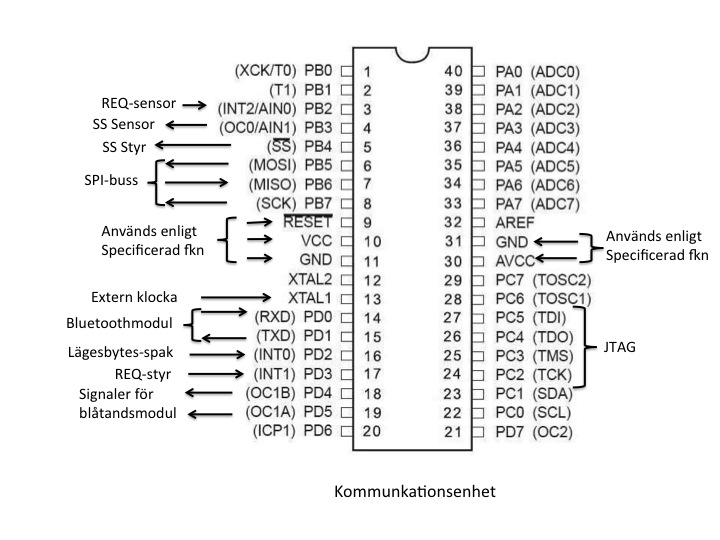
\includegraphics[angle=0,scale=0.5]{bilder/PIN_komm.jpg}
  \caption{Kommunikationsenhetens pin-anslutningar}
  \label{fig:PINkomm}
\end{figure}

\subsection{Bluetooth}
Todo: Blatand.

\subsection{SPI}
\label{sec:SPI}
SPI bussen är ett kommunikationssystem som använder ett så kallat 
Master-Slav system. I robotens SPI-buss är kommunikationsenheten ensam Master.
SPI-bussen har två slavar i form av styrenheten och sensorenheten. För att 
ställa in huruvida en enhet ska agera master eller slav modifieras på Atmega16 
innehållet i kontrollregistrer för SPI-bussen, SPCR. SPI-bussen arbetar alltid 
i så kallat full duplex läge vilket betyder att överföringar kan ske i två 
riktningar samtidigt. Alla överföringar i systemet sker med två bytes åt 
gången, en headerbyte som bland annat innehåller adressen och en databyte. 
När kommunikationsenheten avslutat en överföring så analyseras alltid 
headerbyten, som mottagits genom tvåvägskommunikationen, innan nästa 
överföring behandlas.  


Robotens kommunikationssystem fungerar så att styr- och sensorenheten har 
möjlighet att ta initiativ till överföringar till och från 
kommunikationsenheten. Detta är inte standard på SPI-bussen utan löses med två 
stycken extrasignaler, så kallade Request-signaler. Alla sorters kommunikation 
kommer att styras med hjälp av avbrott, vilket är ett utmärkt sätt att hantera 
plötsliga externa kommandon. Då någon av slavarna vill påbörja en överföring 
sätts enhetens REQ signal hög, vilket genererar ett avbrott hos mastern. Är 
mastern upptagen då en hög REQ signal skickas så får enheten vänta på att 
mastern avslutat den pågående överföringen. Efter att mastern blivit 
uppmärksammad om att en överföring efterfrågas sätts SS-signalen till den 
berörda enheten låg. Överföringen startas i det ögonblick som mastern skriver 
något till det temporära SPI-registret, SPDR. I detta ögonblick så börjar 
mastern också dela ut en klockpuls för överföringen till slavarna. I detta 
läge och framåt görs ingen skillnad på huruvida det var slaven eller mastern 
som initierade överföringen. Alla SPI-överföringar avslutas med att en speciell
avbrottsflagga, kallad SPIF, sätts. När detta sker kommer båda parterna i 
överföringen att spara undan den mottagna datan. Då alla SPI överföringar sker 
med 8 bitar upprepas denna procedur två gånger för varje överföring.

Nedan följer klargöranden om hur de olika portarna i SPI-bussen används, samt 
vilka register som används och hur dessa programmeras. 

\subsubsection{SPI-bussens portar}

Atmel Atmega16 har hårdvarustöd för SPI-bussar. Detta betyder i praktiken att 
det finns pinnar på processorn som enkelt kan ställas in för att fungera 
enligt SPI-standard. Dessa pinnar ligger alla på Port B, se \ref{fig:PINkomm}.
I \ref{fig:spibuss} visas hur pinnarna i de olika enheterna ska kopplas samman.

\begin{figure}[H]
  \centering
 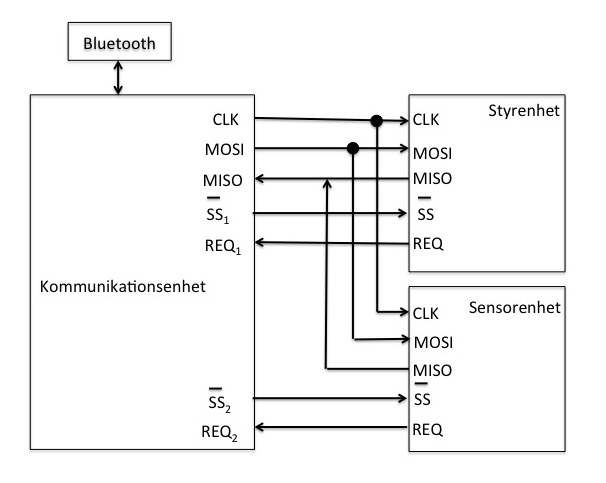
\includegraphics[angle=0,scale=0.5]{bilder/SPI-buss.png}
  \caption{SPI-bussens olika anslutningar. }
  \label{fig:spibuss}
\end{figure}


\textbf{SCK}


SCK porten är en port som förmedlar en klocka med en viss frekvens från 
mastern till de två slavarna. Denna signal bestämmer hur snabbt överföringen 
ska ske. Klockan kommer börjar skickas då mastern skriver något till dess 
temporära SPI dataregister, SPDR. När detta skett skickas totalt 8 pulser 
vilket överför 8 bitar i båda riktningar. Mastern och slavarna måste 
konfigureras för att överföringens olika skeden ska ske samtidigt i 
klockcykeln. Robotens enhet är konfigurerade för att börja med överföring av 
MSB i det temporära SPI-registret SPDR. SCK signalen är konfigurerad till att 
vara låg då ingen överföring sker.

I robotens SPI-buss används frekvensen 4 MHz, det vill säga 1/4-del av 
enheternas arbetsklockan på 16 MHz, för överföringar. Detta är den snabbast 
möjliga överföringshastigheten som garanteras av tillverkaren Atmel. Vid 
behov finns också möjlighet att öka överföringshastigheten till halva 
arbetsklockan, det vill säga 8 MHz. Märk dock att denna överföringshastighet 
inte är garanterad att fungera för slavar.


\textbf{MOSI}


MOSI porten är den port som används när kommunikationsenheten ska skicka 
information till styrenheten och sensorenheten. Den kommer alltså att 
användas som input för slavarna och output för mastern. MOSI-signalen 
parallellkopplas till slavarna, se \ref(fig:spibuss). Om SPI-bussen är 
korrekt inställd kommer slaven som inte är avsedd att motta den skickade 
datan att ignorera vad överföringen. Se pin SS för mer information om 
denna funktion.

\textbf{MISO}


MISO porten används då kommunikationsenheten hämtar information från styr- 
och sensorenheten. Den är alltså att vara en input för mastern och output för 
båda slavarna. Precis som MOSI-signalen porten är MISO-signalerna 
parallellkopplade till slavarna.  Då all kommunikation med SPI är tvåsidig 
används även MOSI porten varje gång MISO porten används och viceversa. En 
slav som inte är vald genom en hög SS-signal, se nedan, kommer inte 
att kunna skicka något via MISO-porten. 

\textbf{SS}
\label{sec:SS}


SS portarna skickar eller tar emot en variant på en chip-select signal. Den SS
-signal som är låg väljer vilken av slavarna som mastern ska kommunicera med. 
Endast en av de två SS signalerna får vara låg samtidigt, detta för att 
undvika busskonflikter. Dessa portar kommer att vara output på mastern(
kommuikationsenheten) och input på styr- och sensorenheten(slavarna).

En låg SS signal hos någon av slavarna betyder att slavens SPI är aktiverad, 
förutsatt att nödvändiga bitar satts i slavens SPI-kontrollregister 
SPCR. Överföringen kommer inte att startas förens mastern skriver data till 
dess temporära dataregister SPDR. Överöringens start genererar inget avbrott 
hos slaven, utan sker istället parallellt med övrig aktivitet hos slaven. Då 
överföringen avslutats genereras ett avbrott där slaven sparar undan den 
skickade byten. Detta avbrott initieras genom att flaggan SPIF sätts hög. En 
enhet som får en hög SS signal kommer att ha sin SPI inaktiv och kommer inte 
att påverkas av aktivitet på databussen. Efter att två bytes överförts sätts 
SS signalen åter hög och mastern påbörjar en analys av den skickade headern 
och om denna specificerar att den mottagna datan ska skickas någonstans.

\textbf{REQ}


REQ portarna används av styr- och sensorenheten för att uppmärksamma 
kommunikationsenheten om att de har ny data att förmedla. När 
kommunikationsenheten tar emot en hög signal på någon av REQ portarna kommer 
det att generera ett avbrott. Detta möjliggörs genom att REQ-signalerna är 
inkopplade till portar på kommunikationsenheten som kan programmeras till att 
generera avbrott vid förändringar. Under avbrottet kommer SS signalen till 
enheten som begärt kommunikation att sättas låg och kommunikationen påbörjas. 
Då mastern kan vara upptagen i det ögonblick då den mottar en hög REQ-signal 
så låter slavarna REQ-signalen vara hög tills dess att överföringen är färdig 
då den sätts låg.

REQ-signalen används också för att bekräfta att slavarna sparat undan en 
headerbyte och är redo att ta emot en databyte. 

\subsubsection{SPI-register på Atmega16}

Det finns i Atmega16 flertalet register som används för att kontrollera SPI-
bussen. Dessa register varierar lite i funktion beroende på om processorn är 
inställd för att fungera som master eller slav på SPI-bussen. För mer 
information om dessa register se *INSERT KÄLLA atmega16 guide*

\textbf{SPI Statusregister - SPSR}


Detta register innehåller dels två olika flaggor och dels en bit som kan 
sättas hög för att fördubbla SPI-bussens överföringshastighet om processorn 
är konfigurerad till att fungera som master . 

MSB är SPIF-flaggan som sätts hög på både master och slav när en 
SPI- överföring slutförts. Tillåts SPI-avbrott kommer 
det att leda till ett avbrott i processorn när denna flagga sätts hög. 
Flaggan rensas genom att denna avbrottsvektor utförs, alternativt genom att 
SPSR läses och därefter läsa från(eller skriva till) SPI-bussens data-register SPDR.

Resten av registrets innehåll används inte i projektet.

\textbf{SPI kontrollregister - SPCR}


Innehållet i detta register avgör om och hur SPI-bussen ska fungera på 
processorn. Endast de bitar som konfigureras i roboten kommer att beskrivas. 
Värt att notera är att robotens överföringshastighet, 1/4 av arbetsklockan, 
uppnås genom att de två minst signifikanta bitarna lämnas låga.

Bit 7 sätts hög för att tillåta avbrott då SPIF sätts hög. Denna bit är satt 
på alla enheter på roboten.

Bit 6 sätts hög för att använda SPI-buss. Sätts inte denna bit hög kommer 
inte SPI-överföringar att fungera.

Bit 4 sätts hög för att göra enheten till master. Det betyder att denna bit 
ska vara hög på kommunikationsenheten men låg på styr- och sensorenheten.

\textbf{SPI dataregister- SPDR}


Detta är ett temporärt 8-bits dataregister som skiftas vid en SPI-överföring. 
Slavar kan skriva till SPDR vid godtyckligt tillfälle. Då mastern skriver 
till SPDR påbörjas överföringen. Då varje överföring i roboten består av två 
skiftningar av SPDR är det viktigt att informationen i SPDR sparas mellan de 
två skiftningarna.


\subsubsection{Exempel}

För att tydliggöra hur bussen fungerar beskrivs nedan ett exempel på hur en 
överföring kan gå till.

När roboten befinner sig i labyrint-läge har sensorenheten gjort en ny 
avläsning som resulterar i beslutet att en 90\degree kurva är nödvändig. Den 
vill distribuera denna information vidare till både styrenheten och PCn som 
övervakar robotens aktivitet. Sensorenheten sätter då en hög utsignal på sin 
REQ port vilket resulterar i ett avbrott på kommunikationsenheten. 
Kommunikationsenheten är för närvarande är för närvarande upptagen med 
överföring av reglerdata till styrenheten, så avbrottet får vänta tills det 
att denna överföring är klar. Under denna väntan är sensorenhetens REQ signal 
fortsatt hög.

I avbrottet på kommunikationsenheten så sätts SS signalen till sensorenheten 
låg, och därefter förmedlar kommunikationsenheten en klockpuls till 
sensorenheten. När två bytes överförts, en headerbyte och en databyte, så 
avslutas överföringen och SS signalen till sensorenheten sätts åter hög. 
Efter att headerbyten tolkats så sätter kommunikationsenheten SS signalen 
till styrenheten låg, samt genererar en klockpuls till styrenheten. När 
överföringen av två bytes är färdig sätts SS signalen till styrenheten 
återigen hög vilket avslutar överföringen via SPI-bussen. 

Då headerbyten innehöll information om att detta var ett styrbeslut så ska 
kommunikationsenheten också skicka detta till PCn. Detta görs via en UART 
port på kommunikationsenheten efter det att headern som skickats från 
styrenheten analyserats. Det är mycket viktigt att en enhet som inte har 
något att skicka vidare sätter innehållet 

De olika enheternas roll i detta exempel åskådliggörs nedan i ett schema, se 
figur \ref{fig:schema}.


\begin{figure}[H]
 \centering
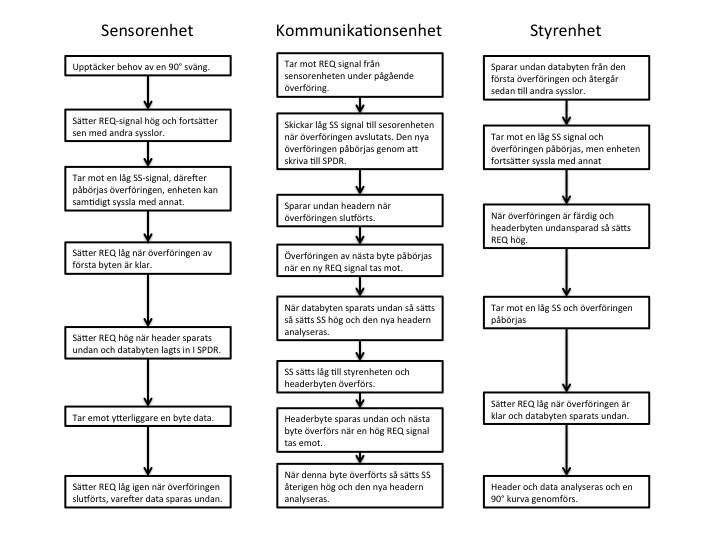
\includegraphics[angle=0,scale=0.7]{bilder/schema_exempel.jpg}
  \caption{Schema över de olika enheternas metodik vid exempelöverföringen}
  \label{fig:schema}
\end{figure}



